\documentclass[Measurements]{subfiles}
\begin{document}
\section{Measurements}
\label{sec:Measurements}

\subsection{Expermimental setup}
Based on the \ac{CMS} popularity measurements of March 1st by w3techs \footnote{\url{http://w3techs.com/technologies/overview/content_management/all}}, Wordpress is chosen as the web application. According to their survey, 17,4 \% of all web servers run Wordpress and it holds 54,6 \% of the CMS market share. Wordpress has, by far, the greatests market share and is therefore a popular target for cyber criminals.

\subsection{Testing framework}
As there is no standard set of rules for performance testing web servers, the described definition aims at being, what in medicine is called, a gold standard test~\cite{wacholder1993validation}. This comprises that the test environment as close as possible mimics a real life situation. \\ 
In order to The following things are vital to performance testing:

\begin{description} 
 \item[server-side] text 
 \item[client-side] text
\end{description}

\begin{figure}[h]
\caption{Experimental setup}
\centering
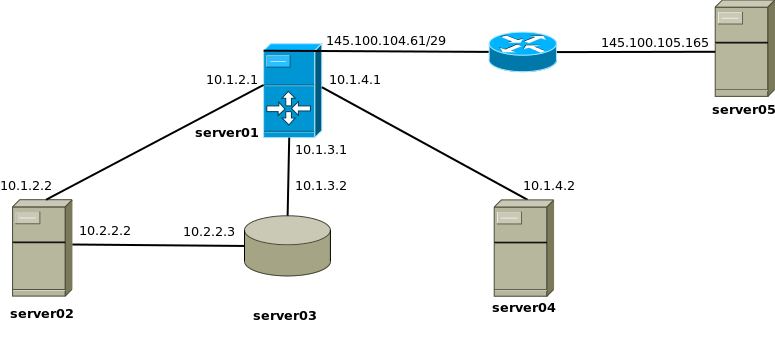
\includegraphics[scale=0.4] {images/infrastructure.png}
\label{fig:Experimental setup}
\end{figure}


\end{document}

